\subsection{Les \emph{newsgroups}}
\label{newsgroups}
\subsubsection{Pr\'esentation}
Le BR fournit aux \'el\`eves un service de \emph{newsgroups}, souvent surnomm\'e \guillemotleft~les br~\guillemotright . Ils fonctionnent un peu comme un
forum : chacun peut poster une annonce, poser une question,
 r\'epondre \`a  un sujet post\'e par un autre \'el\`eve, \ldots 
Ils sont tr\`es utiles pour faire de la pub pour une activit\'e
organis\'ee par un binet, poser une question en cas de probl\`eme, ou
tout simplement savoir ce qu'il se passe sur le plat\^al. Pour qu'ils
puissent remplir pleinement ce r\^ole, le BR a \'edict\'e un certain
nombre de r\`egles que les newsmestres sont charg\'es de faire
respecter.

\subsubsection{Les diff\'erents \emph{newsgroups} de frankiz}
Frankiz h\'eberge un grand nombre de \emph{newsgroups} (plus de 200), mais il est probable qu'ils ne t'int\'eressent pas tous.
Nous te conseillons vivement de t'abonner aux br suivants :

\begin{itemize}
\item[\ngname{br.eleves} :] posts g\'en\'eraux (pas de petites annonces, br.pa est l\`a  pour \c ca ! ), int\'eressant potentiellement un grand nombre d'\'el\`eves. C'est \guillemotleft{}~\textsc{le}~\guillemotright{} br que tu dois lire;

\item[\ngname{br.eleves.evenements} :] le br qui annonce tous les \'ev\`enements importants \`a  venir : c'est un peu une extension des annonces frankiz;
	 
\item[\ngname{br.pa} :] pour les petites annonces. Tu cherches un bidule: tu \'ecris \guillemotleft{}~Ping Bidule~\guillemotright{}. Tu as en a ta possession un machin que tu veux rendre \`a  son propr\'etaire, vendre, partager, etc. : tu \'ecris \guillemotleft{}~Pong Machin~\guillemotright{}. C'est \guillemotleft{}~\textsc{le}~\guillemotright{} lieu, et le seul, pour les annonces;

%\smallskip

%Rappel : \`a  un ping correspond \guillemotleft{}~Je cherche~\guillemotright{}, \`a  un pong \guillemotleft{}~J'ai trouv\'e~\guillemotright{} ou \guillemotleft{}~J'ai~\guillemotright{}.

%\smallskip


\item[\ngname{br.promo.ta\_promo} :] pour les posts ne concernant \emph{a priori} qu'une seule promo (Rouje, J\^one ou Oranje);
	 
\item[\ngname{br.enseignement.*} :] pour tout ce qui a trait \`a  l'enseignement (un DM, un message aux d\'el\'egu\'es d'enseignement, \dots) concernant ta promo (Rouje ou Jone) ou l'ensemble des \'el\`eves;
 
\item[\ngname{br.section.ta\_section\_sportive} :] le \emph{newsgroup} de ta section. Utile pour savoir ce qu'il s'y passe et planifier les activit\'es;

\item[\ngname{br.binet.br} :] comme son nom l'indique, il s'agit du \emph{newsgroup} du binet r\'eseau. \`A utiliser pour les questions ayant un lien \emph{direct} avec le BR;

\item[\ngname{br.kes} :] le \emph{newsgroup} de la K\`es. Il sert essentiellement \`a  la K\`es pour faire une annonce ou aux \'el\`eves pour poser une question aux kessiers (note: il n'est pas non plus interdit de se d\'eplacer \`a  la K\`es pour poser ta question directement).

\end{itemize}



Pour le reste, voila une liste de quelques \emph{newsgroups} utiles :
\begin{itemize}

\item[\ngname{br.informatique.windows/linux/mac} :] selon ton OS, quand tu as un probl\`eme, besoin d'une astuce, ou d'un logiciel;

\item[\ngname{br.informatique.media.request.*} :] pour les films, les musiques ou autre;

\item[\ngname{br.informatique.media.nouveautes} :] pour les derniers films, s\'eries, albums;

\item[\ngname{br.binet.ton\_binet} :] chaque binet a son \emph{newsgroup} (s'il en a demand\'e un). Il sert le plus souvent pour la communication interne du binet, ses annonces ou \`a  poser une question au dit binet. Dans le cas d'un nouveau binet, le BR peut lui cr\'eer un \emph{newsgroup}, mais uniquement apr\`es que le binet a \'et\'e cr\'e\'e dans les r\`egles \`a  la K\`es;

\item[\ngname{br.binet.polemix} :] le forum pour \emph{troller} (un \emph{troll} est une tr\`es longue discussion qui d\'eg\'en\`ere) par excellence;
                          
\item[\ngname{br.communaut\'e.*} :] les \emph{newsgroups} de diff\'erentes communaut\'es (religieuses, musicales, g\'eographiques ou autres);

\item[\ngname{br.test} :] quand tu veux tester un truc sur les \emph{newsgroups}, viens le faire ici plut\^ot que de pourrir un br utile. La tradition est d'y laisser une blague apr\`es y avoir post\'e.

\end{itemize}


Il arrive parfois que certains \emph{newsgroups} temporaires soient cr\'e\'es pour des \'ev\'enements particuliers (campagne K\`es). Leur cr\'eation sera annonc\'ee
le plus souvent sur \fkz ou sur le \ngname{br.eleves}.

\subsubsection{Les r\`egles}
\textbf{Utilisation des diff\'erents \emph{newsgroups}}
\begin{itemize}

 \item Pas de posts \`a  la fois sur \ngname{br.promo.jone} et \ngname{br.promo.rouje} : ces posts vont sur \ngname{br.eleves} car concernent les deux promotions \`a  la fois;
 \item Ne pas faire de posts en double : faire des \emph{crossposts}, les messages non crosspost\'es seront supprim\'es (et vous aurez droit \`a  un RTFIBRp11);
 \item Pas de posts sur tous les \ngname{br.section} \`a  la fois : \c ca concerne l'ensemble des \'el\`eves;
 \item Eviter les trolls sur \ngname{br.eleves} : essayer au maximum d'aller sur \ngname{br.binet.polemix} (quitte \`a  initier la discussion par un \emph{crosspost} depuis le \ngname{br.eleves});
 \item Pas de ping/pong sur le \ngname{br.eleves} : le \ngname{br.pa} est l\`a  pour \c ca, pas besoin d'en rajouter sur le \ngname{br.eleves}. Les messages essayant de contourner cette r\`egle (du genre \guillemotleft{}~p ing~\guillemotright{}) seront supprim\'es;
 \item Comme son nom l'indique, le \ngname{br.eleves} concerne tous les \'el\`eves, donc avant de poster, demande toi si un autre br ne serait pas plus adapt\'e, et ne ciblerait pas plus sp\'ecifiquement les personnes \`a  qui tu veux faire passer le message. D'une mani\`ere g\'en\'erale, r\'efl\'echis \`a  l'endroit o\`u tu dois poster.

\end{itemize}

\textbf{R\`egles des messages}
\begin{itemize}
 \item Pas de caract\`eres sp\'eciaux en surnombre pour le titre (\#, *, \$ ou autres);
 \item Pas de lettres capitales en surnombre dans le titre (les majuscules et les sigles sont suffisants);
 \item Les r\`egles habituelles de discussions sur des forums sont en vigueur, \`a  savoir \'eviter le langage SMS, rester poli, pas de propos racistes, xenophobes ou insultants. N'agissez pas comme vous n'aimeriez pas qu'on vous parle face \`a  face;
 \item Il vaut mieux garder son calme : une explication face \`a  face arrange les choses beaucoup mieux que plusieurs messages d'insulte.
\end{itemize}

\textbf{Mod\'eration par les newsmestres}
\begin{itemize}
 \item Les newsmestres ne mod\`erent pas tous les br; en cas de probl\`eme sur un \ngname{br.binet} ou un \ngname{br.section} quelconque, les utilisateurs sont invit\'es \`a  en parler aux newsmestres, \`a  \mail{news@eleves.polytechnique.fr};
 \item L'usurpation d'identit\'e est interdite et sera sanctionn\'ee par un bannissement des br. Nous rappelons aux utilisateurs qu'il est possible de savoir depuis quelle adresse IP un message a \'et\'e post\'e. Poster depuis un ordinateur de binet ou de bar section est ainsi fortement d\'econseill\'e (sauf sur les \ngname{br.binet.*} ou \ngname{br.section.*} correspondants, mais mettre son nom en fin de message reste conseill\'e et poli);
 \item Les newsmestres sont les membres du BR charg\'es de l'administration et de la mod\'eration des \emph{newsgroups}. Leur but est de maintenir les \emph{newsgroups} dans un \'etat correct, pour que tout le monde puisse en profiter et trouver ce qu'il y cherche. Ne prends donc pas une remarque de leur part comme une attaque personnelle. Ce sont des gens comme les autres, ils s'efforcent de maintenir l'ordre dans la limite de leur possible, en suivant des r\`egles au maximum coh\'erentes; les insulter ne fera pas avancer les choses, au contraire;
 \item Tout utilisateur abusant du non-respect des r\`egles et/ou de la patience des newsmestres sera banni d'abord en \'ecriture, puis en lecture, pour une dur\'ee d'au moins 24\,h.
\end{itemize}



\subsubsection{Poster sur plusieurs \emph{newsgroups}\dots }



Il se peut qu'un jour tu veuilles annoncer un grand \'ev\'enement sur les \emph{newsgroups}, et que pour ceci tu aies envie de poster ton message sur
plusieurs \emph{newsgroups}. Alors avant de commencer \`a  poster sur un \emph{newsgroup}, faire copier-coller, poster sur le \emph{newsgroup} suivant,
etc., lis ce qui suit et apprends \`a  gagner du temps et \`a  simplifier ta vie et celle de tes camarades.

\begin{description}

\item[Qu'est-ce qu'un \emph{crosspost} ?]
Un \emph{crosspost} permet de poster le m\^eme message sur diff\'erents \emph{newsgroups}, et de renvoyer toutes les r\'eponses sur le m\^eme \emph{newsgroup}, quel
que soit le \emph{newsgroup} sur lequel elles ont \'et\'e post\'ees.

\item[Avantage d'un \emph{crosspost}]
\begin{itemize}
 \item Toutes les r\'eponses que les gens te font sont centralis\'ees sur le m\^eme forum,
       ce qui t'\'evite de perdre du temps \`a  lire des r\'eponses diss\'emin\'ees
       sur les diff\'erents forums o\`u tu as post\'e.
       De plus, ceux qui te r\'epondent peuvent eux aussi lire facilement toutes les r\'eponses
       que tu as d\'ej\`a  re\c cues;
 \item Sur certains clients \emph{news}, il suffit de lire le message post\'e sur un forum
       pour qu'il soit marqu\'e comme lu sur tous les autres forums o\`u il a \'et\'e post\'e,
       ce qui \'evite ainsi aux gens de devoir lire plusieurs fois le m\^eme message;
 \item Cela t'\'evite de recevoir comme r\'eponse un \guillemotleft~RTFIBRp11~\footnote{Read The Fucking InfoBR page 11 : Lis Le Putain d'InfoBR page 11. Pour des raisons historiques, le \emph{cross-post} est d\'ecrit \`a  la page~11 de l'InfoBR, c'est-\`a -dire cette page.}~\guillemotright  hargneux de la part d'un(e) newsmestre.
\end{itemize}

\item[Comment faire un \emph{crosspost} ?]
Il suffit de mettre dans le premier en-t\^ete (\menu{Groupe de discussion} ou \emph{Newsgroup}) la liste de tous les \emph{newsgroups} o\`u tu veux
poster, s\'epar\'es par des virgules. Exemple : \ngname{br.eleves, br.lose, br.binet.bob, br.promo.rouje}.

Il faut ensuite mettre dans l'en-t\^ete \menu{Transf\'erer \`a } (ou \menu{Follow-up to}) le \menu{newsgroup} o\`u tu veux que les r\'eponses apparaissent. Si
tu n'a pas ces en-t\^ete, sous \app{Outlook Express} va dans \menu{Affichage} et clique sur \menu{Tous les en-t\^etes} quand tu \'ecris ton message; sous
\app{Thunderbird}, clique sur la gauche de la deuxi\`eme ligne et s\'electionne \lien{Faire suivre \`a  :} dans le petit menu d\'eroulant. Attention, ce doit \^etre
l'un des \emph{newsgroups} o\`u tu postes le message.
Voir par exemple les captures d'\'ecran pour \app{Thunderbird} et \app{Outlook Express}.\\

\noindent
\begin{minipage}{0.44\textwidth}
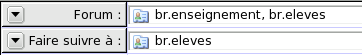
\includegraphics[width=0.98\textwidth]{images/cross_post_TB}
\end{minipage}
\begin{minipage}{0.44\textwidth}

\includegraphics[width=0.98\textwidth]{images/cross_post_OE}
\end{minipage}


C'est bien plus simple que d'envoyer successivement ton message sur tous les \emph{newsgroups}, et la centralisation des r\'eponses permet de conserver
un peu de clart\'e sur les \emph{newsgroups} tout en te facilitant la vie. Que des avantages donc!

\end{description}

\subsubsection{Autres \emph{newsgroups}}
Le site \urllink{polytechnique.org} dispose de son propre service de \emph{newsgroups}. Il sont
accessibles \`a  tous les polytechniciens, qu'ils soient actuellement sur le campus ou membres de
promos pr\'ec\'edentes. Pour plus d'informations, consulte \urllink{www.polytechnique.org}.

